\documentclass[]{article}

\usepackage[italian]{babel}
\usepackage[margin=20mm, footskip = 20pt]{geometry}
\usepackage{array}
\usepackage{tabularx}
\usepackage{graphicx}
\usepackage{subfiles}
\usepackage{hyperref}
\usepackage{nameref}
\usepackage{titlesec}
\usepackage{longtable}
\usepackage[table]{xcolor}
\usepackage{titling}
\usepackage{lastpage}
\usepackage{ifthen}
\usepackage{calc}
\usepackage{soulutf8}
\usepackage{contour}
\usepackage{float}
\usepackage{fancyhdr}
\usepackage{multirow}
\usepackage{pgfgantt}
\usepackage{lscape}

\newcommand{\hr}{\par\vspace{-.1\ht\strutbox}\noindent\hrulefill\par}

\graphicspath{ {./}
	{./commons/res}
}

%--------------------------------------------------
% Comandi per inserire contenuto del documento
%--------------------------------------------------
\makeatletter

\newcommand\appendToGraphicsPath[1]{%
	\g@addto@macro\Ginput@path{{#1}}%
}

\newcommand{\setTitle}[1]{%
	\newcommand{\@phTitle}{#1}%
}
\newcommand{\phTitle}{\@phTitle}

\newcommand{\setDate}[1]{%
	\newcommand{\@phDate}{#1}%
}
\newcommand{\phDate}{\@phDate}

\newcommand{\setUso}[1]{%
	\newcommand{\@uso}{#1}%
}
\newcommand{\uso}{\@uso}

\newcommand{\setVersione}[1]{%
	\newcommand{\@versione}{#1}%
}
\newcommand{\versione}{\@versione}

\newcommand{\disabilitaVersione}{%
	\renewcommand{\setVersione}[1]{}%
	\renewcommand{\versione}{DISABILITATA}
}

\newcommand{\setResponsabile}[1]{%
	\newcommand{\@responsabile}{#1}%
}
\newcommand{\responsabile}{\@responsabile}

\newcommand{\setRedattori}[1]{%
	\newcommand{\@redattori}{#1}%
}
\newcommand{\redattori}{\@redattori}

\newcommand{\setVerificatori}[1]{%
	\newcommand{\@verificatori}{#1}%
}
\newcommand{\verificatori}{\@verificatori}

\newcommand{\setModifiche}[1]{%
	\newcommand{\@modifiche}{#1}%
}
\newcommand{\modifiche}{\@modifiche}

\makeatother 

%--------------------------------------------------
% Comandi per i documenti esterni e il glossario
%--------------------------------------------------

\newcommand{\dext}[1]{\textsc{#1\textsubscript{\textit{D}}}}

\newcommand{\glock}[1]{\textsc{#1\textsubscript{\textit{G}}}}

%--------------------------------------------------
% Comandi per impostare sottotitoli di quarto e quinto livello
%--------------------------------------------------

\setcounter{secnumdepth}{4}
\setcounter{tocdepth}{4}

\titleformat{\paragraph}
{\normalfont\normalsize\bfseries}{\theparagraph}{1em}{}
\titlespacing*{\paragraph}{0pt}{2.25ex plus 1ex minus .2ex}{1.5ex plus .2ex}

\titleformat{\subparagraph}
{\normalfont\normalsize\bfseries}{\thesubparagraph}{1em}{}
\titlespacing*{\subparagraph}{0pt}{1.75ex plus 1ex minus .2ex}{.75ex plus .1ex}

\appendToGraphicsPath{../../commons/res/}


%------------------------------
%
% COMANDI DI CONFIGURAZIONE
%
%------------------------------

\setTitle{Allegato Tecnico}

\setVersione{1.0.0}

\setDate{15-04-2021}

\setResponsabile{Lucia Fenu}

\setRedattori{
	Alessandro Dindinelli \\&
	Valton Tahiraj \\&
}

\setVerificatori{
	Lucia Fenu \\&
}

\setUso{Esterno}

\setModifiche{
	DA TOGLIERE IF POSSIBOL :) & DA TOGLIERE IF POSSIBOL :) & DA TOGLIERE IF POSSIBOL :) & DA TOGLIERE IF POSSIBOL :) & DA TOGLIERE IF POSSIBOL :) \\
}

\begin{document}

	% Direttive per la creazione del titolo tramite comando maketitle
\title{\huge \textsc{\phTitle{}} \\
	\vspace{11pt} \large \textsc{\phDate{}}}

\author{} % Non toccare
\date{} % Non toccare

%--------------------
% Frontespizio
%--------------------

% Logo del gruppo
\begin{figure}[t!]
	\centering
	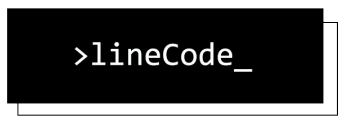
\includegraphics[width=20em]{lclong}
\end{figure}

% Titolo / Nome
\maketitle
\thispagestyle{empty}

% Dati specifici sul doc in forma tabulare
\begin{table}[ht]
	\begin{center}
		\label{tab:Dati sul documento}
		\begin{tabular}{r|l}
			\multicolumn{2}{c}{ \textsc{Dati sul documento} } \\
			\hline
			\textbf{Versione} & \versione{} \\
			\textbf{Uso} & \uso{}  \\
			\textbf{Redattori} & \redattori{} \\
			\textbf{Verificatori} & \verificatori{} \\
			\textbf{Responsabile} & \responsabile{} \\
			\textbf{Destinatari} & lineCode \\
								& prof.\ Vardanega Tullio \\		
								& prof.\ Cardin Riccardo \\
			\ifthenelse{\equal{\uso}{Esterno}}{
								& Sanmarco Informatica
			}{} \\
		\end{tabular}
	\end{center}
\end{table}

\newpage

\renewcommand{\arraystretch}{2} % allarga le righe con dello spazio sotto e sopra
\begin{longtable}[H]{>{\centering\bfseries}m{2cm} >{\centering}m{3.5cm} >{\centering}m{2.5cm} >{\centering}m{3cm} >{\centering\arraybackslash}m{5cm}}
	\rowcolor{lightgray}
	{\textbf{Versione}} & {\textbf{Nominativo}} & {\textbf{Ruolo}} & {\textbf{Data}} & {\textbf{Descrizione}}  \\
	\endfirsthead%
	\rowcolor{lightgray}
	{\textbf{Versione}} & {\textbf{Nominativo}}  & {\textbf{Ruolo}} & {\textbf{Data}} & {\textbf{Descrizione}}  \\
	\endhead%
	\modifiche{}%
\end{longtable}
	\newpage
	\tableofcontents
	\newpage
	\listoffigures
	\listoftables
	\newpage
	%--------------------------------
	%
	% IL CONTENUTO INIZIA DA QUI
	%
	%--------------------------------

	\section{Introduzione}
	\subsection{Scopo del documento}
Il documento ha lo scopo di definire le guidelines del way of working adottato dal team lineCode. Le attività presenti in questo documento sono redatte da processi contenuti nello standard ISO/IEC 12207:1995. Risulta quindi necessario che tutti i membri del gruppo prendano visione di questo documento ai fini di coesione e uniformità all'interno del progetto.

\subsection{Scopo del prodotto}
Il \glock{capitolato} C5 ha come obbiettivo la realizzazione di un applicativo \glock{Real-Time} in grado di guidare delle unità dotate di mobilità autonoma in ambienti specifici, partendo dal presupposto che queste si muovano in ambienti in cui sono presenti altre unità (autonome o meno).

\subsection{Glossario e documenti esterni}
In supporto alla documentazione viene fornito un glossario per chiarire, con una definizione, eventuali termini specifici contenuti in questo documento.
Saranno adottati quindi questi due simboli a pedice:
\begin{itemize}
	\item \textit{D} se indicano un documento specifico;
	\item \textit{G} se incluse nel \dext{glossario}.
\end{itemize}

\subsection{Riferimenti}
	\subsubsection{Riferimenti normativi}
	\begin{itemize}
		\item \textbf{{C5 - PORTACS}}: \url{https://www.math.unipd.it/~tullio/IS-1/2020/Progetto/C5.pdf};
        \item \textbf{Oracle Java Code Conventions}: \url{https://www.oracle.com/technetwork/java/codeconventions-150003.pdf};
        \item \textbf{Angular coding style guide}: \url{https://angular.io/guide/styleguide}.
	\end{itemize}
	\subsubsection{Riferimenti informativi}
	\begin{itemize}
		\item \textbf{ISO/IEC 12207:1995}: \url{https://www.math.unipd.it/~tullio/IS-1/2009/Approfondimenti/ISO_12207-1995.pdf};
		\item \textbf{Gitflow}: \url{http://nvie.com/posts/a-successful-git-branching-model/};
		\item \textbf{Documentazione Zapier}: \url{https://zapier.com/help};
		\item \textbf{Documentazione act}: \url{https://github.com/nektos/act/blob/master/README.md};
		\item \textbf{Studio di Fattibilità}: \dext{Studio di Fattibilità v1.0.0};
		\item \textbf{Piano di Qualifica}: \dext{Piano di Qualifica v2.0.0};
		\item \textbf{Piano di Progetto}: \dext{Piano di Progetto v2.0.0}.
	\end{itemize}
	\newpage

	\section{Architettura del prodotto}
	\subsection{Descrizione generale}
Durante la fase di progettazione, il gruppo \textit{lineCode} ha deciso di modellare la struttura del prodotto in quattro componenti distinte:
\begin{itemize}
	\item \textbf{server}: motore di calcolo che coordina le unità e genera le informazioni per la UI. Viene modellato seguendo la \textit{layered architecture};
	\item \textbf{interfaccia grafica}: mostra la mappa e permette di gestire le unità e gli utenti. Viene modellato seguendo il \textit{MVVM};
	\item \textbf{unità}: si occupa di simulare il comportamento di un'unità all'interno dell'ambiente. Viene modellato seguendo la \textit{hexagonal architecture};
	\item \textbf{sensori}: si occupa di simulare il comportamento dei sensori delle unità all'interno dell'ambiente. Non viene modellato secondo una architettura specifica poiché triviale.
\end{itemize}
La UI e l'unità comunicano con il server tramite l'uso di \glock{WebSocket} e lo scambio di messaggi \glock{JSON}. Il server, quindi, conoscendo la posizione di tutte le unità e ostacoli, genera il percorso migliore e lo comunica alle unità richiedenti e aggiorna la mappa informando l'interfaccia grafica.\\

	\newpage
	
	\subsection{Architettura del server}
	Il pattern architetturale applicato alla componente server è la \textit{Layered Architecture}. \\
Si è scelto tale pattern, sia perché lo si è ritenuto il più adatto a strutturare questo componente sia perchè, se la progettazione architetturale è stata fatta correttamente, i componenti del gruppo potranno lavorare su diversi layer autonomamente. \\
\newline
Di seguito viene illustrato il diagramma dei package.
%\begin{figure}[H!]
%	\centering
%	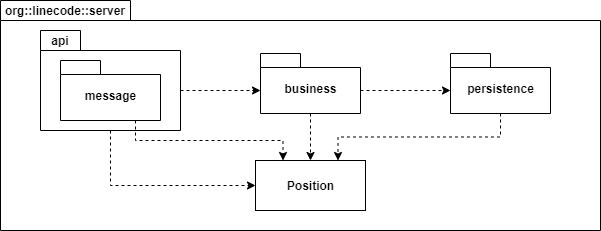
\includegraphics[width=10cm]{images/server_package.png}
%	\caption{Server - Diagramma dei package}
%\end{figure}

\subsubsection{Diagrammi delle classi}

\paragraph{Presentation layer}
Il server copre un ruolo centrale nell'applicazione, comunicando sia con le unità, che con l'interfaccia grafica. Qui infatti troviamo i metodi che permettono la gestione della connessione alle altre componenti del sistema, e quindi anche l'invio e la ricezione di messaggi. A tale scopo sono previste opportune interfacce.

\paragraph{Business layer}
Qui troviamo la logica per la gestione dei dati in entrata ed uscita dal server. \\
Per garantire l'indipendenza dal layer sovrastante, la comunicazione verrà implementata con un sistema di segnali e slot. Il business layer emetterà degli opportuni segnali che verranno intercettati dal layer sovrastante, ma la ricezione degli stessi non sarà di sua preoccupazione.

\paragraph{Persistence layer}
Per immagazzinare i dati  in uso all'applicazione, vengono utilizzate tre interfacce, per mappa, utenti ed unità, che vengono poi implementate in SQLite.

\paragraph{Messages}
Per garantire i principi \textit{separation of concerns} e \textit{layer isolation}, sono state implementate delle interfacce allo scopo di essere gli oggetti di comunicazione tra i layer stessi.

% QUI I DIAGRAMMI VARI DI CLASSE
%\begin{landscape}
%	\begin{figure}[h!]
%		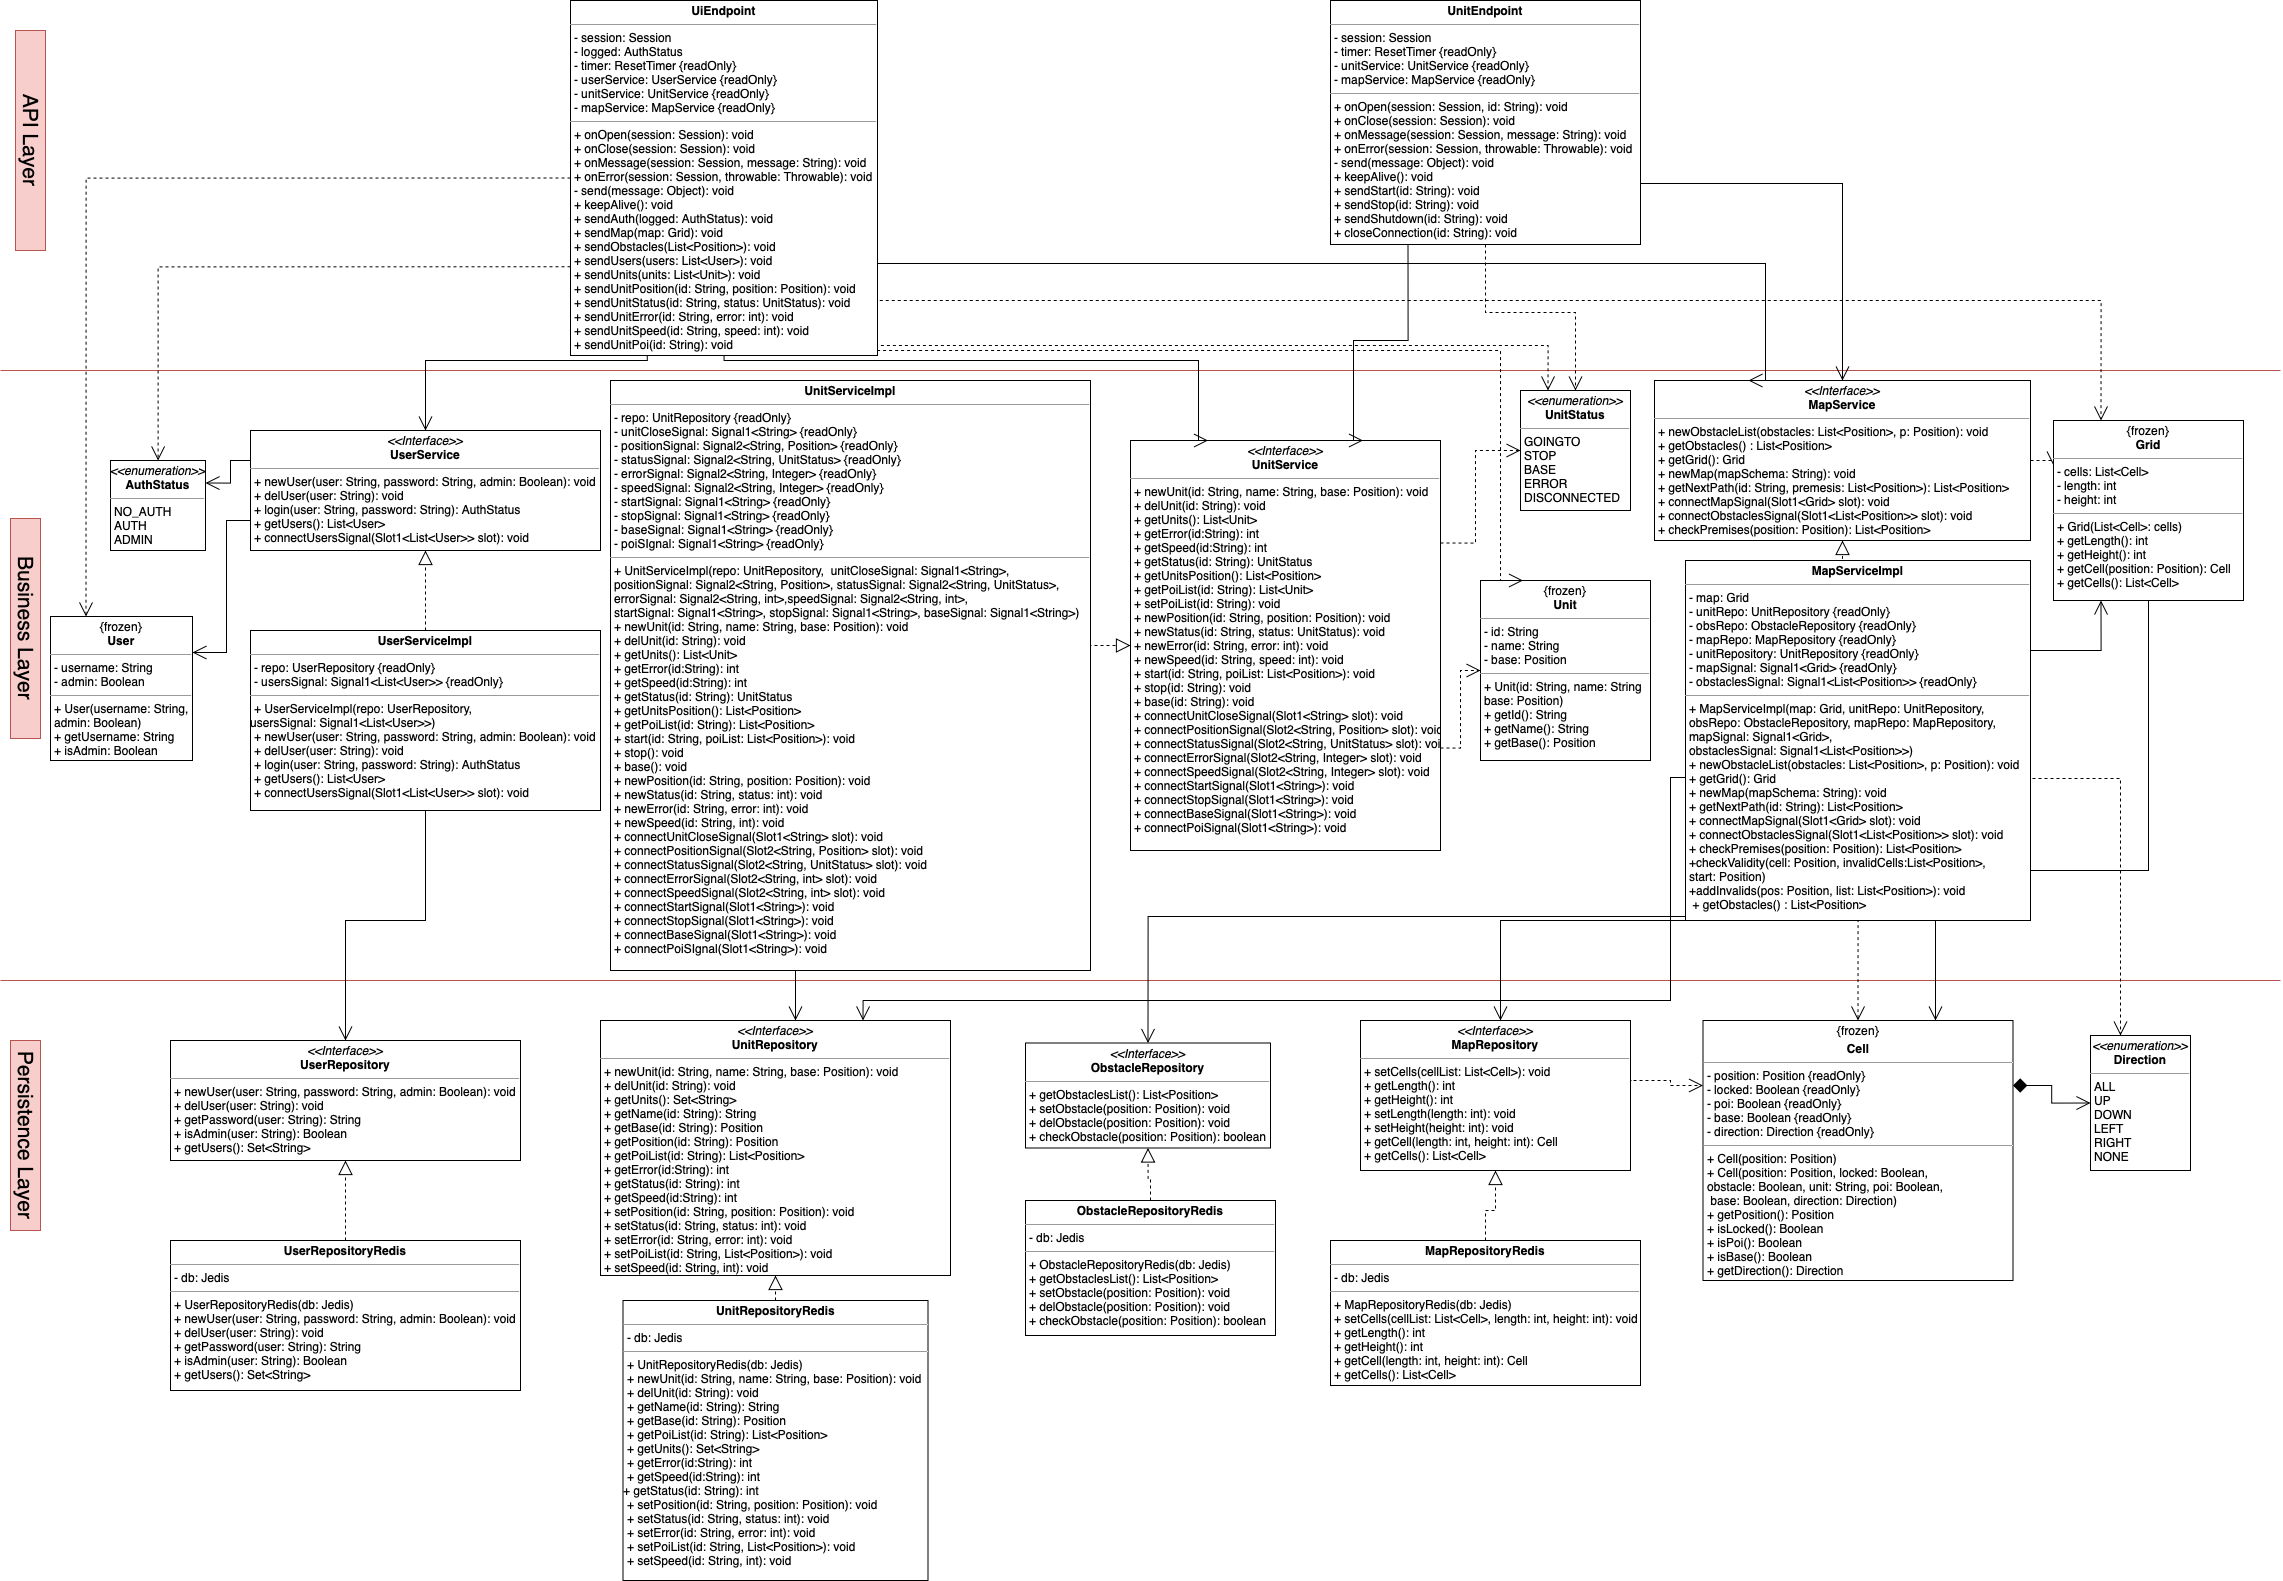
\includegraphics[width=24cm]{images/server_classi.png}
%		\caption{Server - Diagramma delle classi}
%	\end{figure}
%\end{landscape}

\paragraph{Database layer}
I dati che verranno immagazzinati nel database avranno la seguente struttura:
% QUI immagine del db layer
%\begin{figure}[H!]
%	\centering
%	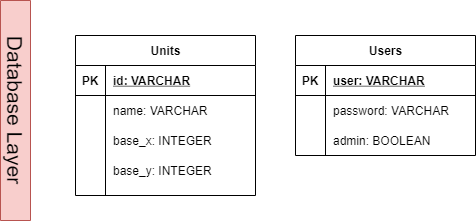
\includegraphics[width=10cm]{images/server_dblayer.png}
%	\caption{Server - Database layer}
%\end{figure}

\subsubsection{Diagrammi di sequenza}
Mini descrizione dello scenario del diagramma
%\begin{figure}[H!]
%	\centering
%	\includegraphics[width=10cm]{images/server_sequenza.png}
%	\caption{Server - Diagramma di sequenza}
%\end{figure}
	\newpage
	
	\subsection{Architettura dell'interfaccia}
	L'interfaccia grafica è realizzata tramite il framework \glock{Angular}, quindi il design architetturale utilizzato è il \textit{Model View ViewModel} (\textit{MVVM}) che è intrinseco nel framework stesso. \\
La comunicazione con il server avviene tramite \glock{WebSocket} e dunque asincrono. Viene sfruttato il design pattern \textit{Observer} per permettere un'aggiornamento asincrono dei componenti dell'interfaccia.\\
Inoltre, per garantire l'estensibilità del codice, il servizio \textit{WebSocketService} implementa l'interfaccia \textit{ServerService} che mette a disposizione i metodi per interfacciarsi con il server. In questo modo un cambio di tecnologia, ad esempio passando a richieste \glock{Http}; non comporterebbe uno stravolgimento dell'architettura. \\
Per lo stesso motivo sono previste delle interfacce per rappresentare i vari tipi di messaggi che vengono ricevuti dal server, che vengono successivamente implementate per specificarne le caratteristiche. \\
Per garantire che ogni componente riceva solo i dati di suo interesse, vengono utilizzate delle classi definite da utente per rappresentare la trasmissione delle informazioni tra i componenti. \\
Si è pianificato di avere un componente per ogni funzionalità(O ALTRA PAROLA?) principale che l'interfaccia mette a disposizione all'utente. \\
\newline
Di seguito l'architettura dell'interfaccia viene rappresentata tramite due diagrammi delle classi: il primo per descrivere il \textit{Model}, e quindi le modalità con cui i messaggi vengono inviati e ricevuti dal server, ed il secondo, per il \textit{Viewmodel} che rappresenta la struttura dei vari \glock{Angular Components}. La parte di \textit{View} comprende i templates degli \glock{Angular Components}, e quindi la struttura del codice \glock{HTML}. \\


\newpage

\begin{landscape}
	\begin{figure}[h!]
		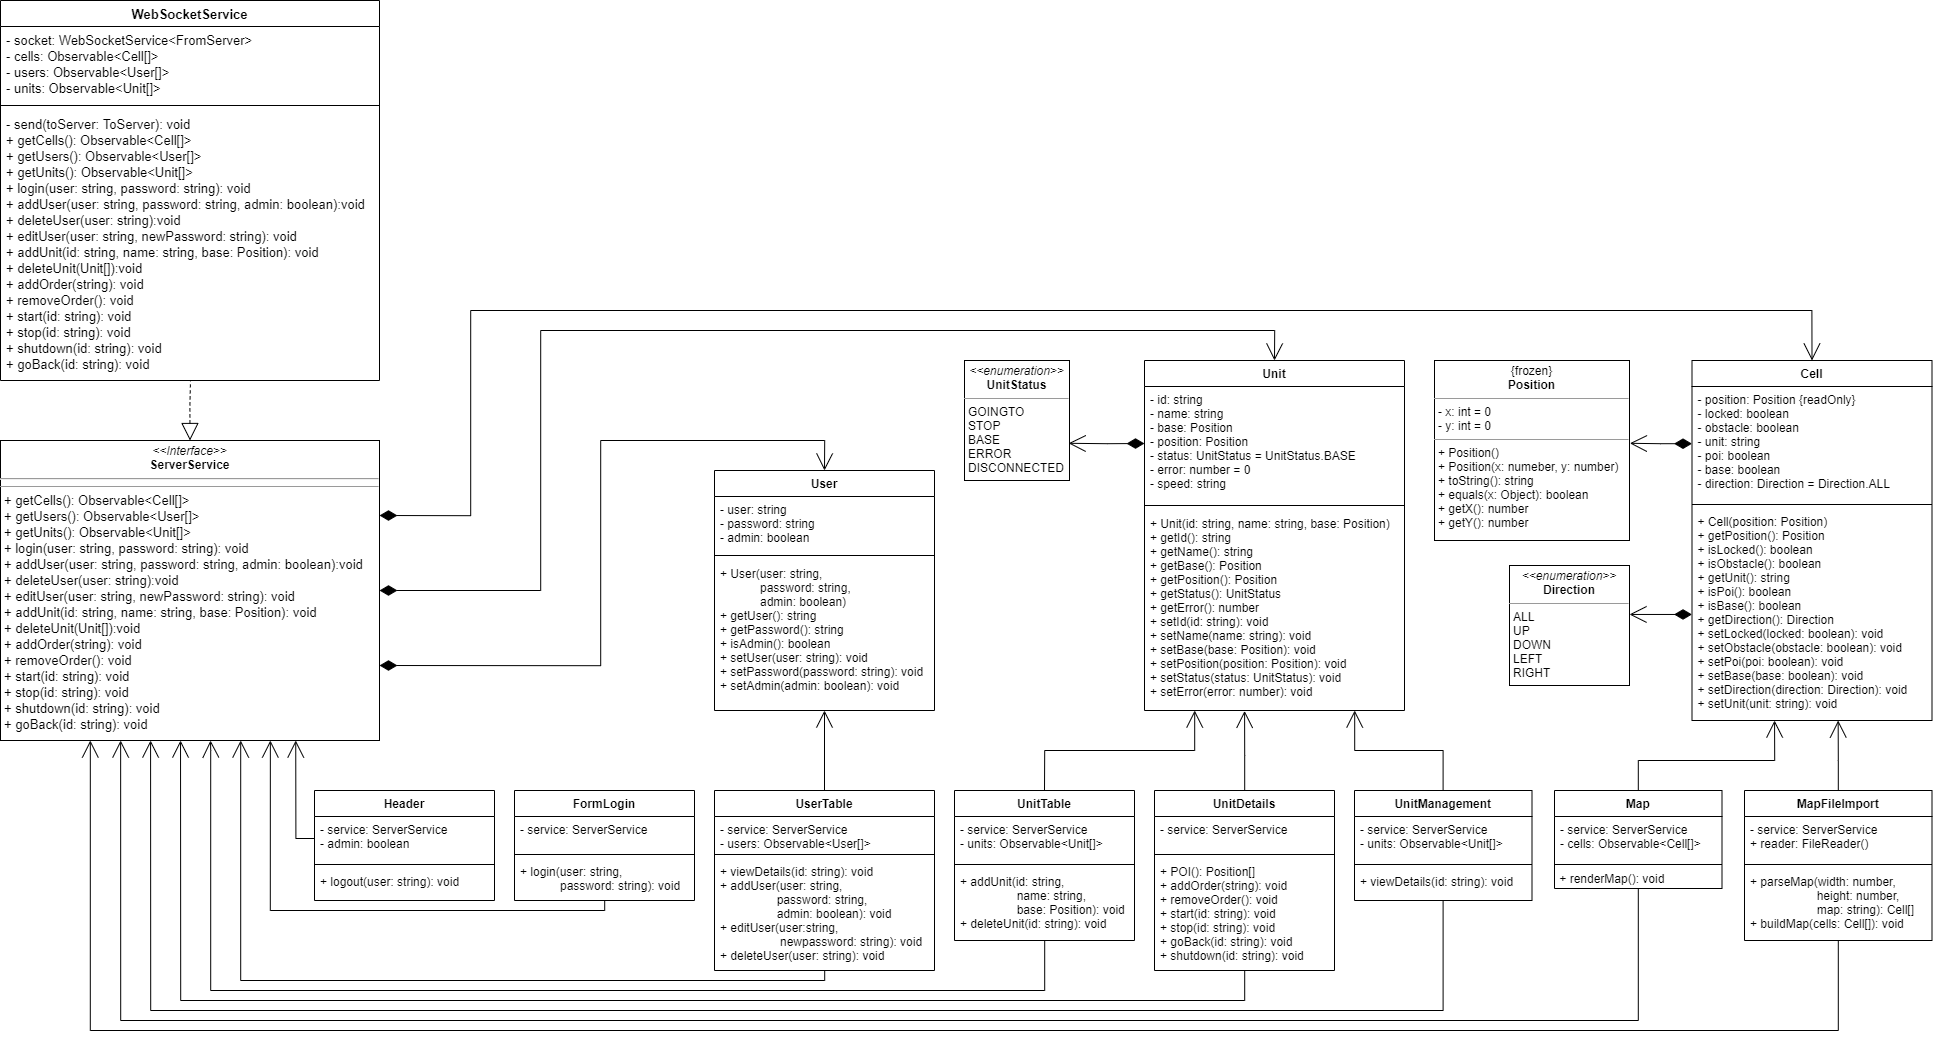
\includegraphics[width=24cm]{img/ui component.png}
		\caption{Architettura dell'interfaccia - View Model}
	\end{figure}
\end{landscape}
\newpage

\begin{landscape}
	\begin{figure}[h!]
		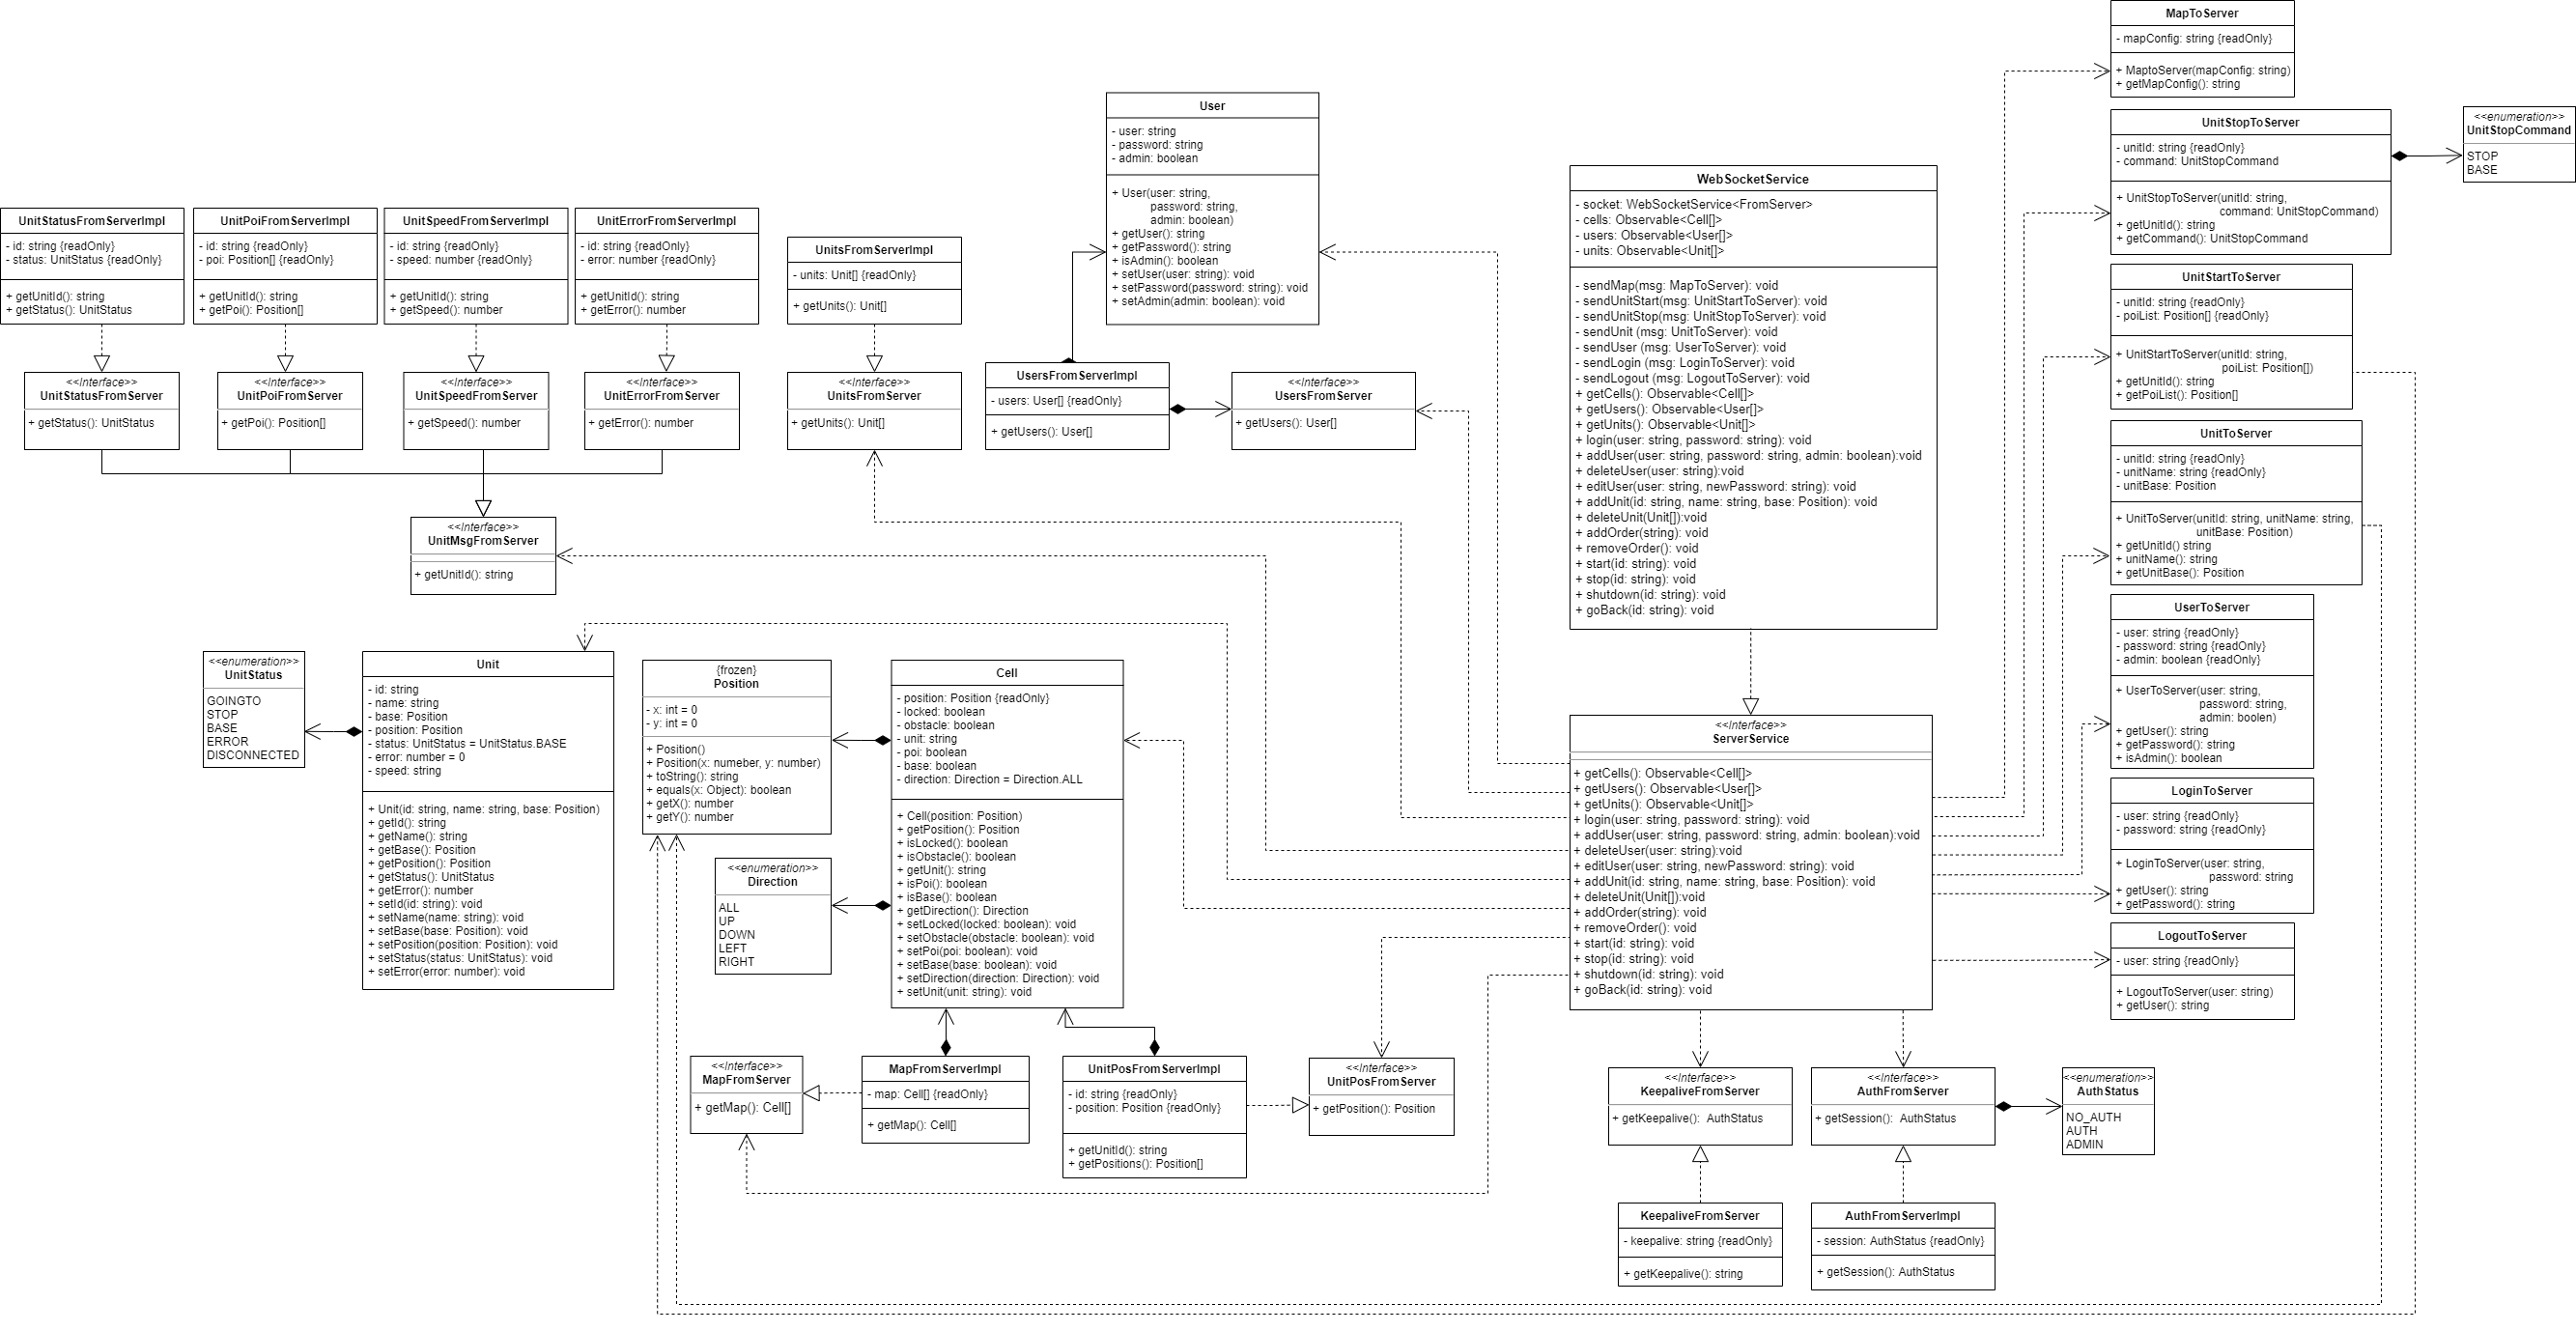
\includegraphics[width=24cm]{img/ui messaggi.png}
		\caption{Architettura dell'interfaccia - Model}
	\end{figure}
\end{landscape}
	\newpage
	
	\subsection{Architettura delle unità}
	\input{res/sez5_arch_unità.tex}
	\newpage
	
\end{document}